\documentclass[../main.tex]{subfiles}
\externaldocument{implementation}
\graphicspath{{\subfix{../images/}}}

\begin{document}

\begin{newrequirements}
    \textbf{Note that this section is a substantial 
    portion of the grade for your final 
    report and will require a significant 
    amount of effort.}

    \begin{todolist}
    \item[\done] describe in detail the tests you have 
        conducted to verify that your prototype 
        satisfies the desired functional 
        requirements while meeting the design 
        constraints. For example, if you used 
        Use Cases to describe your non-
        functional requirements, then for each 
        use case you should write a test case, 
        run it and report the testing results
        (the key test cases can be added as an 
        Appendix). Functional testing will 
        allow you to find defects then fix them 
        and also identify possible 
        improvements.  You need to have a 
        comprehensive set of tests that 
        verifies correct functionality of every 
        component of your system. 

    \item[\done] verify and provide evidence through 
        testing that your solution solved the 
        stated problem and satisfied the 
        requirement specifications and design 
        constraints, documented in Section 3.2 
        of the interim report. If not, explain 
        what is lacking and identify possible 
        improvements 

    \item[\done] This section must present sufficient 
        evidence and clear discussion that your 
        design and prototype met/did-not-meet 
        all of the identified technical and 
        practical constraints documented in 
        Section 3.2. You may use a summary 
        table to elaborate these points. The 
        table columns could contain: 

    \begin{todolist}
    \item Brief description of the constraints 

    \item Explanation of the testing steps taken 
        to evaluate if the constraint was met 
        or not. 

    \item Measurements data that prove your 
        system met/did-not-meet the constraint. 
        Also compare measured data against 
        expected values, then include a \%error 
        as (actual – expected)/expected*100\%, 
        and use only three digits of precision. 
        In case a constraint is not met, then 
        explain the reason for that. 
    \end{todolist}

    \item For further details and examples refer 
        to the document titled ‘Examples of how 
        to address and verify some of the 
        design constraints’ posted on the 
        Senior Projects website. 
         
    \item[\done] Describe in detail the tests performed 
        on the individual subsystems of your 
        project.  Discuss how you tested each 
        subsystem and what the results of each 
        test were. 

    \item In addition, do not forget to include: 

    \begin{todolist}
    \item If you have a GUI of some type, you 
        need a screen shot of it. 

    \item If you have a physical display of some 
        type (LEDs, LCDs, etc.), you need a 
        photograph of the display showing 
        typical operation. 

    \item For any interfaces of your hardware 
        components – USB, I2C, SPI, RS232, 
        parallel interfaces, or A/D inputs – 
        you may show oscilloscope pictures that 
        demonstrate a sample data transfer of 
        this interface and the typical 
        voltage/frequency ranges. 
    \end{todolist}

    \item[\done] You should present the test results, 
        with appropriate level of details in 
        addition to accuracy and completeness, 
        using tables, graphs, diagrams, screen 
        shots etc. Additionally, discuss these 
        results and explain whether the 
        prototype has achieved the 
        requirements. If not state what is 
        lacking or still need improvement then 
        explain the reason for that. There will 
        probably be multiple subsections under 
        this section to describe each system 
        test and its result. 

    \end{todolist}
\end{newrequirements}

\begin{table}[H]
    \centering
    \caption{Summary of the prototype testing}
    \label{tab:testing-summary}
    \begin{tabularx}{\textwidth}{ l X l l l }
        \toprule
        \textit{Constraint} 
            & \textit{Testing procedure} 
                & \textit{Result}
        & \textit{Measurement data} 
            & \textit{Error (\%)} \\

        \midrule
        
        
        ??    & ?? 
        & Met
            & ??
        & 5 \\

        \bottomrule		
    \end{tabularx}
\end{table}

%% Each subsection corresponds to a test.
%% Title the subsection based on the functional requirement OR
%% the design constraint being tested.

% HARDWARE
\subsection{Connecting to the drone}

\lipsum[1]

\subsection{Command-Control system maximum distance}

\lipsum[1]

\subsection{Flying duration \& Batteries}

\lipsum[1]

\subsection{Response time}

\lipsum[1]

\subsection{Payload}

\lipsum[1]

% SOFTWARE
\subsection{\textsc{rl} training}

\begin{table}[H]
    \centering
    \caption{Summary of the \gls{rl} and simulation testing}
    \label{tab:rl-testing-summary}
    \begin{tabularx}{\textwidth}{ X X l X l }
        \toprule
        \textit{Constraint} 
            & \textit{Testing procedure} 
                & \textit{Result}
        & \textit{Measurement data} 
            & \textit{Error (\%)} \\

        \midrule
        
        
        \raggedright Training convergence    
            & Train the agent until the episode rewards converge to a
            value
        & Met
        & Episode rewards converged to around 13 and 8 (for fixed-targets training
        and mobile-targets training respectively)
        & N/A \\
        \addlinespace

        \raggedright Model performance
        & Compare the \gls{rl} agent with random and zig-zag agents
        & Met
        & The \gls{rl} agent performed much better in terms of time
        and energy for fixed-targets and mobile-targets missions
        & N/A \\
        \addlinespace

        \raggedright Drone's height vs. cell width
        & Fly the drone at different heights and record the maximum
        width that it is able to cover
        & Met
        & The regression line manages to fit all point with a
        Pearson's $r$ value of 0.999958
        & 
        \begin{tabular}{l}
            \\
            $1-r^2 =$ \\
            $8.32\times 10^{-3}$ \\
        \end{tabular}
        \\
        % $1-r^2$ \newline $= 8.32\times 10^{-3}$ \\
        \addlinespace

        \bottomrule		
    \end{tabularx}
\end{table}

\subsubsection{Fixed-targets mission}

After 50,000 timesteps of training using the Proximal Policy
Optimization (PPO) algorithm, the average episode reward converged
to around 13 as shown in \cref{fig:episode-rewards-fixed}.
The agent did not achieve the maximum return of 15
on average
due to several reasons. Firstly, the
targets kept changing positions from episode to episode.
Secondly, the softmax output layer of the PPO still produced 
a healthy amount
of exploration away from the targets in some episodes,
and finally, the imperfection in the object detection model made
the agent unable to collect the reward it has received. 
% thinks it moved to a wrong cell when it actually
% did not.
% The Pyzbar library used for object detection has
% an accuracy of up to 90\% in good conditions, but it can 
% be as low as 30\% when the QR code is damaged due to
% an error in photo capturing and processing~\cite{dynamsoft}.

\begin{figure}[!t]
	\centering
	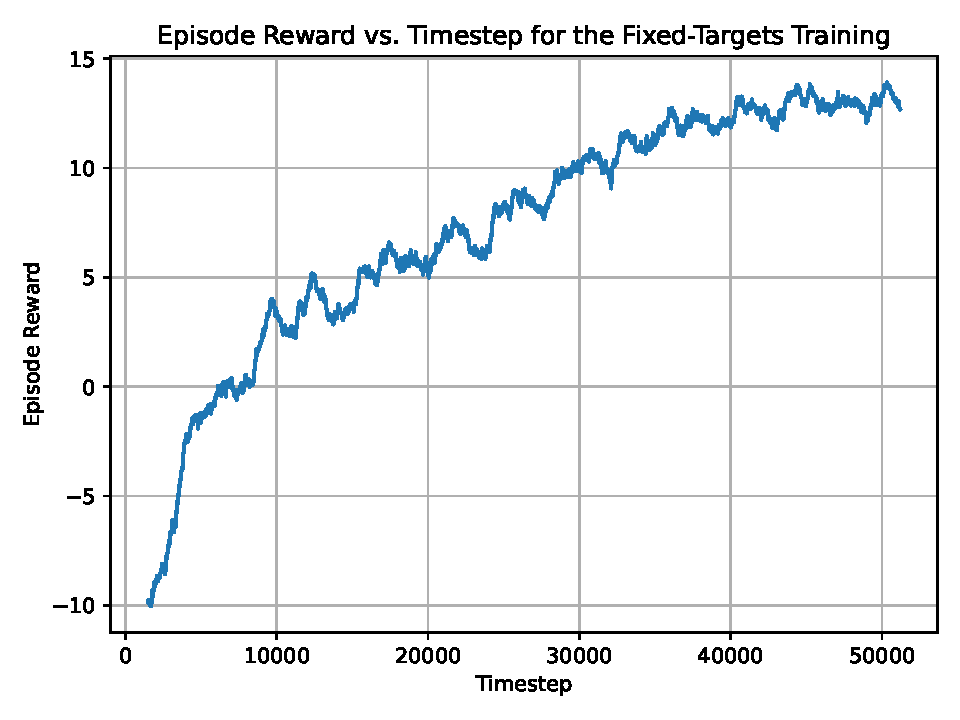
\includegraphics[width=0.8\textwidth]{episode-rewards-fixed}
        \caption{\gls{rl} episode reward convergence during the
        fixed-targets training.}
        \label{fig:episode-rewards-fixed}
\end{figure}

Similarly, \cref{fig:episode-lengths-fixed} shows the the number of
timesteps the agent performed before accomplishing the mission
(visiting all targets) in each episode.
The succesful learning can also be observed here where the agent took
fewer and fewer timesteps as the training was progressing.
It starts at the maximum allowable timestep of 15 and converges at
around 5.

\begin{figure}[!t]
	\centering
	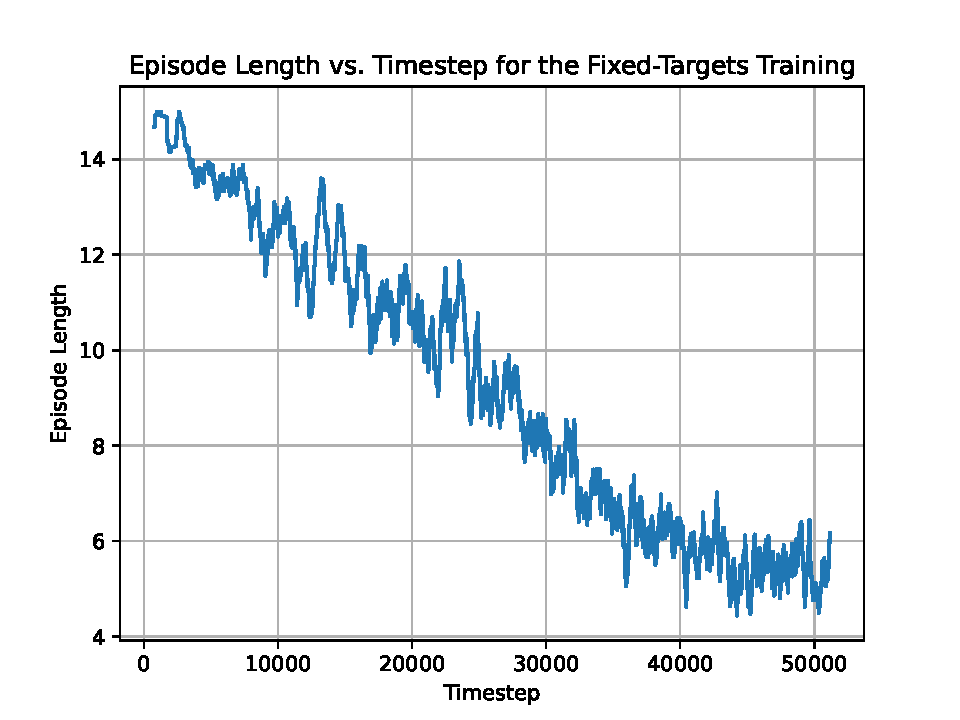
\includegraphics[width=0.8\textwidth]{episode-lengths-fixed}
        \caption{\gls{rl} episode length convergence during the
        fixed-targets training.}
        \label{fig:episode-lengths-fixed}
\end{figure}

\subsubsection{Mobile-targets mission}

As explained in the \cref{sec:implementation}, in this type of
mission, three targets are mobile while the rest are stationary.
The training for this took 100,000 timesteps to achieve conversion as
shown in \cref{fig:episode-rewards-mobile}.
The converged value is around 8, much lower than the static-targets
mission.
This is because the three moving targets added much more complexity in the
learning.

\begin{figure}[!t]
	\centering
	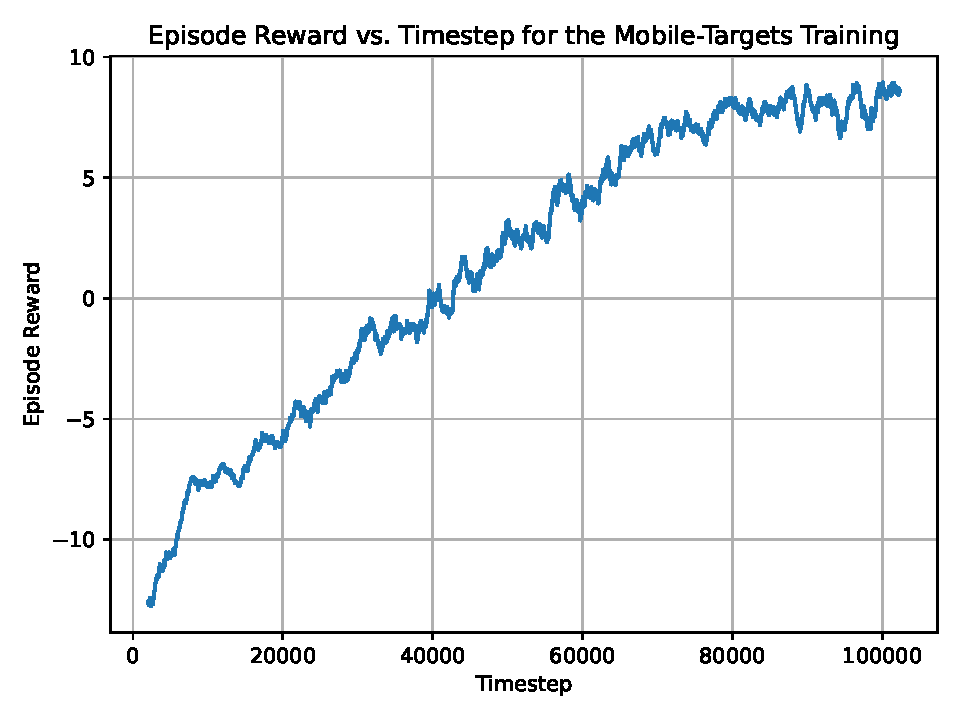
\includegraphics[width=0.8\textwidth]{episode-rewards-mobile}
        \caption{\gls{rl} episode reward convergence during the
        mobile-targets training.}
        \label{fig:episode-rewards-mobile}
\end{figure}

The same trend as the static-targets mission can also be seen in
\cref{fig:episode-lengths-mobile}.
The differences lie in the starting and ending points.
The graph starts at 20 since for this environment, the maximum
timestep was set to be 20 instead of 15 as explained in
\cref{sec:implementation}.
This is to allow the agent to learn effectively in the initial
stages of the training where the agent was more random and the fixed
and mobile targets are located further apart compared to those targets
in the fixed-targets training.
The further distance between these two groups of targets also explains
why the graph converges at 12 timesteps and not 5 as in the
fixed-targets training.

\begin{figure}[!t]
	\centering
	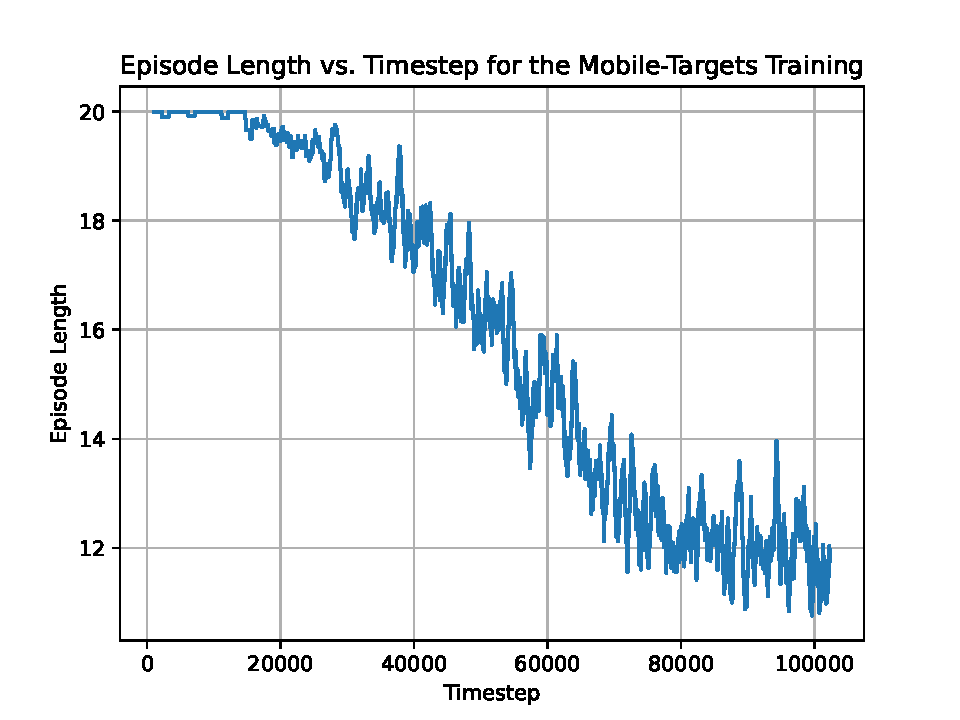
\includegraphics[width=0.8\textwidth]{episode-lengths-mobile}
        \caption{\gls{rl} episode length convergence during the
        mobile-targets training.}
        \label{fig:episode-lengths-mobile}
\end{figure}

\subsection{\gls{rl} model performance}

In order to verify the advantages of an \gls{rl}-trained drone
in the target visitation mission, we have compared it with
two other baseline agents.

The first agent is a drone that completes the same mission 
while moving completely randomly. 
In other words, the probability of taking each of the 
nine available actions is the same.
The second agent moves in a zig-zag manner, as shown
in \cref{fig:zigzag}.
If this zig-zag agent does not visit all the targets the first time
round, it continues from the final cell and follows the same
path as it came but in reverse.
This overall pattern may start from the beginning (cell 1) or 
the end (cell 25).
We have included both variants, named Zigzag1 and Zigzag2
respectively, to make the comparison comprehensive.

\begin{figure}[!t]
	\centering
	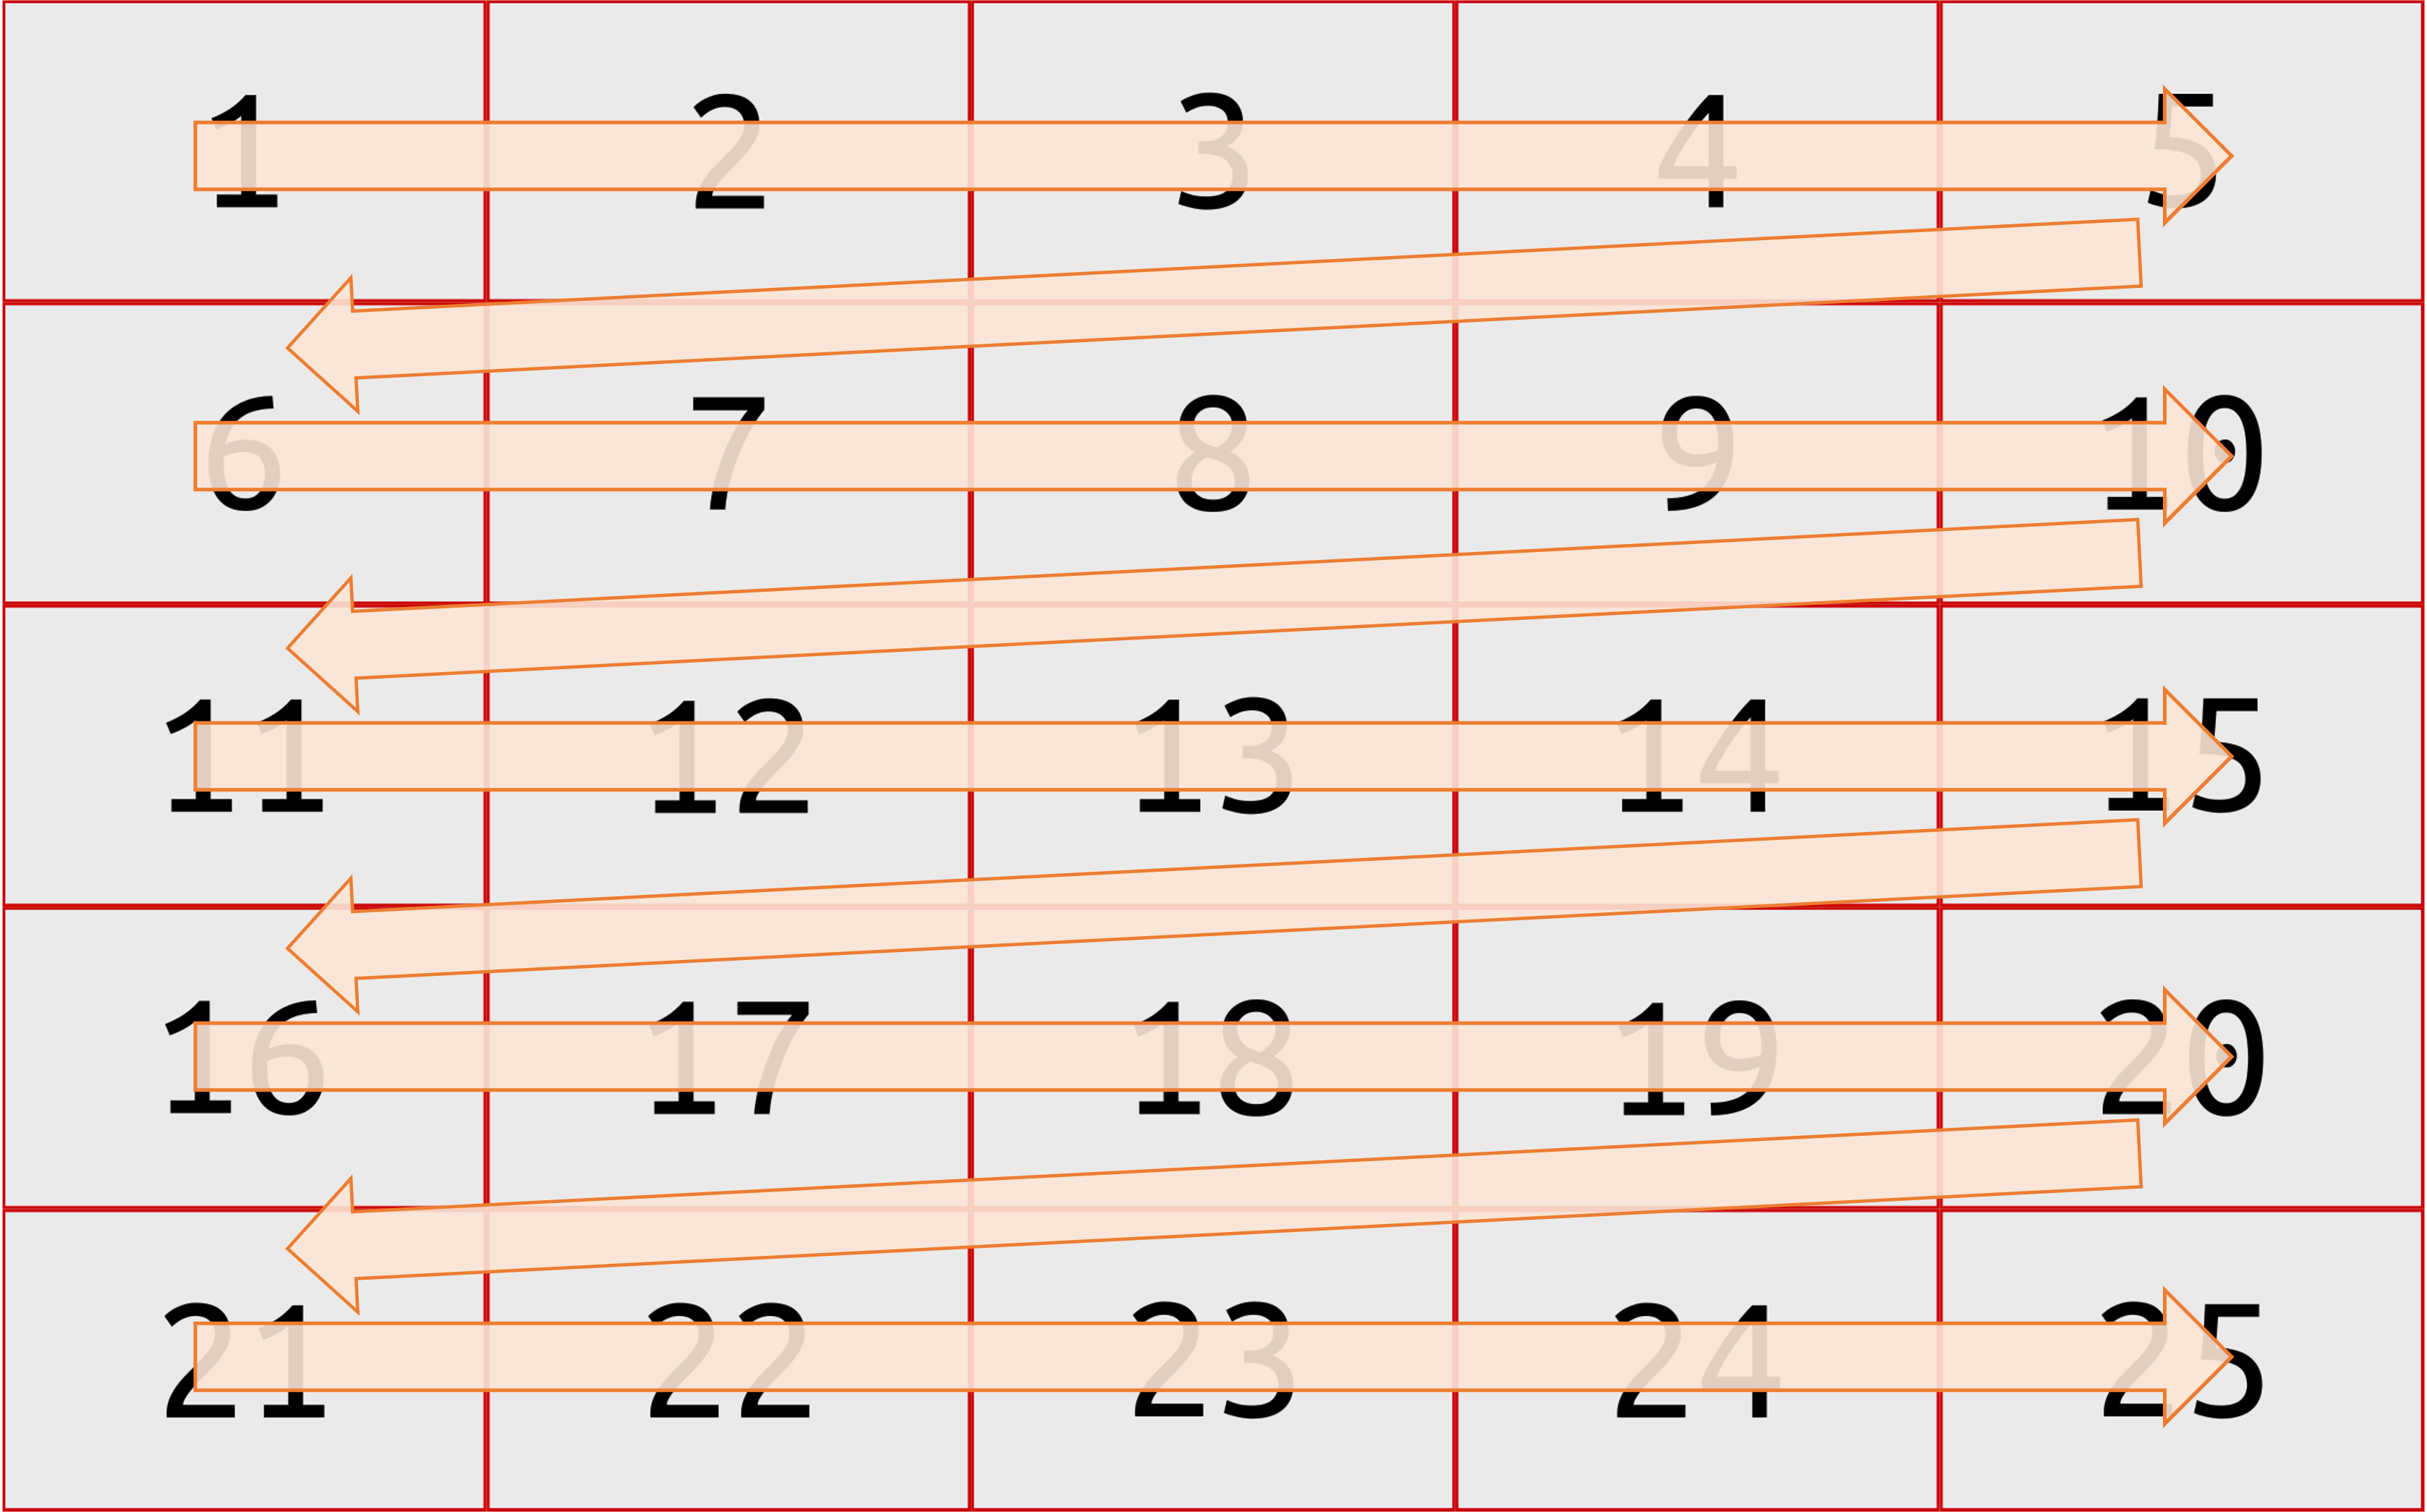
\includegraphics[width=0.8\textwidth]{zigzag}
	\caption{The directions of the drone moving zig-zag
		across the grid according to zigzag-1.
                zigzag-2 begins from cell 25.}
	\label{fig:zigzag}
\end{figure}

To make the comparison objective, 
each of the nine actions executed by random, zig-zag
or \gls{rl} techniques is treated the same way regardless 
of the fluctuations that may arise in the 
distance travelled and speed during
the simulation.
In other words, the distance travelled does not depend
on the technique used but only 
the type of action taken. 
The distances are listed in \cref{tab:distances}.

\begin{table}[tbp]
\caption{The distances travelled by each action based on
    the grid 25x40m\textsuperscript{2} shown in 
    Fig.~\ref{fig:grid}.}
\label{tab:distances}
\centering
\begin{tabular}{p{3.4in} c}
\toprule
Movement directions & Distances, $d$ (m) \\
\midrule
\raggedright Forward-left, forward-right, 
backward-left, backward-right & 9.434 \\
Forward, backward & 5.000 \\
Right, left & 8.000 \\
Starting cell to edge cell e.g. 13\textrightarrow 1 (for zigzag) & 18.868 \\
\raggedright Long diagonal e.g. 5\textrightarrow 6 (for zigzag) & 32.388 \\
\bottomrule
\end{tabular}
\end{table}

On the other hand, the speed is constant for all actions. 
The constant values of speed along with processing time,
and power consumed during movements and hovering
are presented
in \cref{tab:assumptions}
and they are used in the calculations.
Furthermore, since the performance of the agent,
especially the random one, can vary widely and
the positions of the targets are different in each episode, 
10 trials are carried out for each technique and
the average time is taken.

\begin{table}[tbp]
\caption{The values assumed to be constant throughout the
mission.}
\label{tab:assumptions}
\centering
\begin{tabular}{l c c}
\toprule
Parameter & Symbol & Value \\
\midrule
Speed & $v$ & 5 m/s \\
Processing time & $t_{\text{process}}$ & 1 s \\
Hovering time & $t_{\text{hover}}$ & 2 s \\
Power for moving & $P_{\text{move}}$ & 20 W \\
Power for hovering & $P_{\text{hover}}$ & 10 W \\
\bottomrule
\end{tabular}
\end{table}

\Cref{eq:move-time} shows the formula used to
calculate the time taken for a moving action and
\cref{eq:hover-time} for a hovering one.
For the energy, moving actions' consumptions are calculated
by \cref{eq:move-energy} while a hovering one by
\cref{eq:hover-energy}.
\begin{align}
t_{\text{move,tot}} &= 
\frac{d}{v} + t_{\text{process}}
	\label{eq:move-time}
        \\
t_{\text{hover,tot}} &= 
t_{\text{hover}} + t_{\text{process}}
	\label{eq:hover-time}
        \\
E_{\text{move,tot}} &= 
\frac{d}{v} \cdot P_{\text{move}} 
+ t_{\text{process}} \cdot P_{\text{hover}}
	\label{eq:move-energy}
        \\
E_{\text{hover,tot}} &= 
\left( t_{\text{hover}} + t_{\text{process}} \right) \cdot P_{\text{hover}}
	\label{eq:hover-energy}
\end{align}

\subsubsection{Fixed-targets mission}

The results for the fixed-targets mission are presented as bar charts in 
\cref{fig:time-plot-fixed} and \cref{fig:energy-plot-fixed}.
Both of the plots indicate that the \gls{rl} agent completed
the mission in the shortest time and least energy, followed
by the Zigzag2 since it started in an area 
where the probability
distribution of the targets is the highest.
In fact, the \gls{rl} agent is about twice as fast and twice
as energy-saving as Zigzag2.

\begin{figure}[tbp]
	\centering
	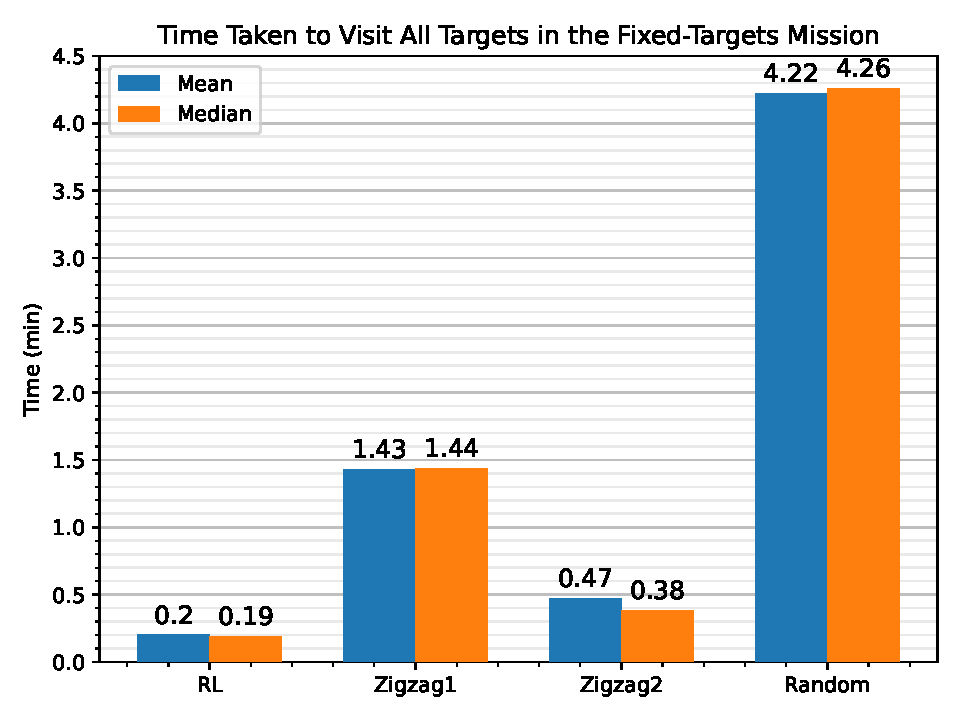
\includegraphics[width=0.8\textwidth]{time-plot-fixed}
	\caption{The time taken by each technique
            to complete the fixed-targets mission showing the mean and
    median.}
        \label{fig:time-plot-fixed}
\end{figure}

\begin{figure}[tbp]
	\centering
	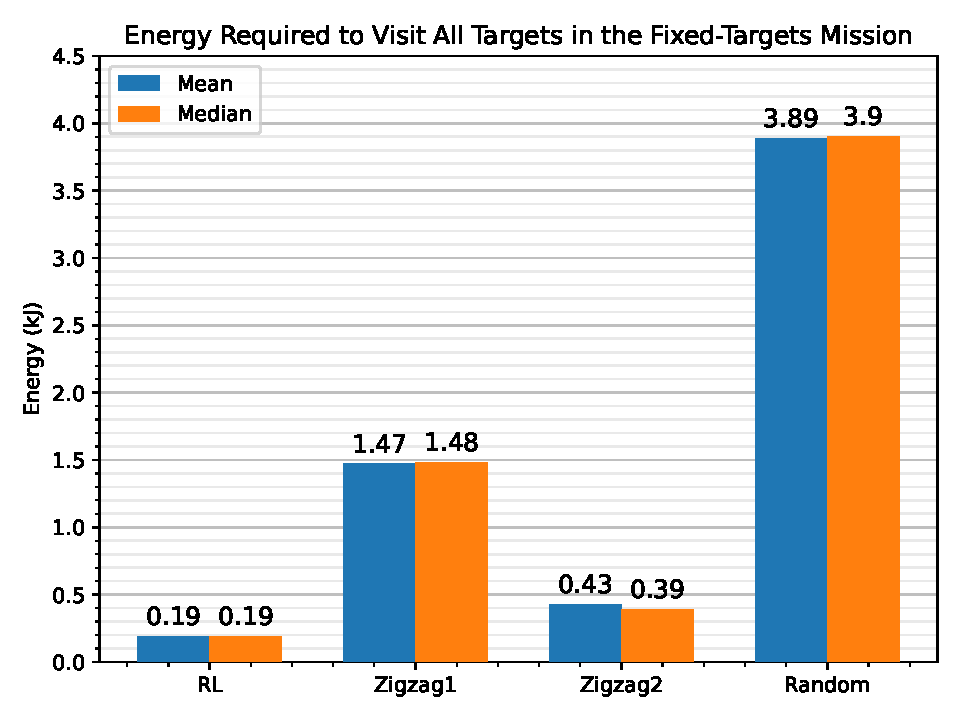
\includegraphics[width=0.8\textwidth]{energy-plot-fixed}
	\caption{The energy consumed by each technique
            to complete the fixed-targets mission showing the mean and
    median.}
        \label{fig:energy-plot-fixed}
\end{figure}

The \gls{rl} performed the best in this environment because
the targets were not placed in a uniform distribution
across the grid,
in which the random agent may have equalled the performance,
neither were they placed deterministically, 
in which case the zig-zag technique with the
right starting point would have won.
Another interesting observation from the comparison is that
the \gls{rl} agent did not execute the hovering action at all
because after so many timesteps choosing to hover and
receiving a reward of -1, it has learnt that it is an
action that is not beneficial in all states.

\subsubsection{Mobile-targets mission}

For the mobile-targets mission, the results for time taken and energy consumed are shown in 
\cref{fig:time-plot-mobile} and \cref{fig:energy-plot-mobile} respectively.
Again, the \gls{rl} agent performed the best, more than two times
faster and more energy-saving than the
second fastest and the second energy-saving agent which is Zigzag2.
Zigzag2 started from cell 25, and by the time it took it to reach
cell 1, the moving targets had already got to their north-west
destination corner and moved within the cell 1 only.

In contrast, Zigzag1 started from cell 1 and in the first round it
missed the moving targets as they moved to the cells already covered
by the Zigzag1 agent.
Therefore, it had to restart scanning in reverse before it
covered all the targets making it much slower than Zigzag2.
As expected, the random agent performed the worst as it did not follow
any particular strategy to visit the targets. It only relied on
chances.

\begin{figure}[tbp]
	\centering
	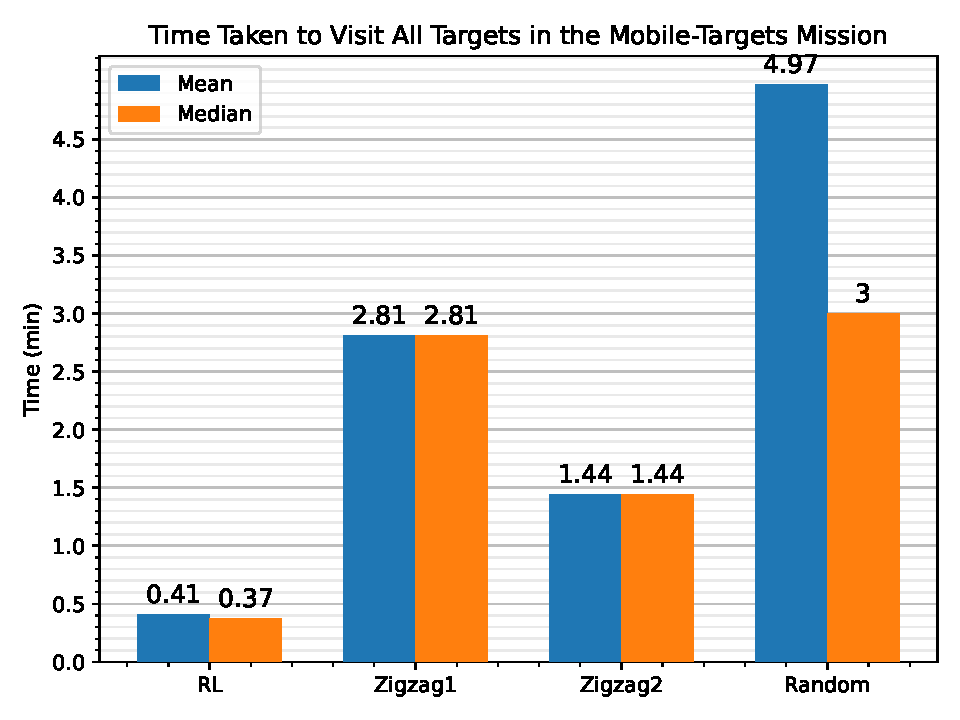
\includegraphics[width=0.8\textwidth]{time-plot-mobile}
	\caption{The time taken by each technique
        to complete the mobile-targets mission showing the mean and
    median.}
        \label{fig:time-plot-mobile}
\end{figure}

\begin{figure}[tbp]
	\centering
	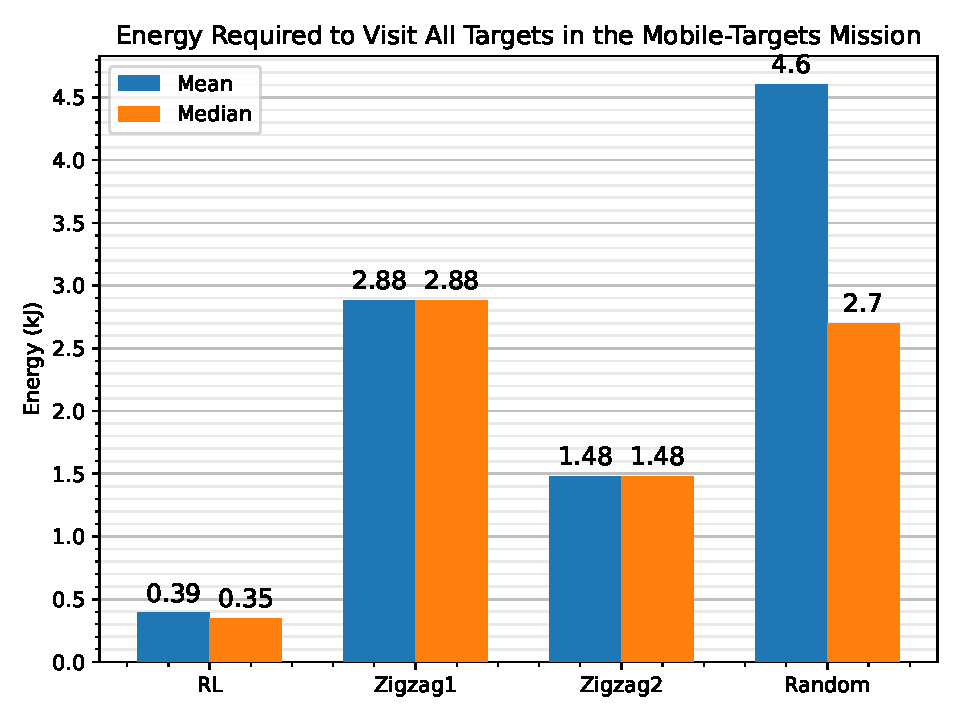
\includegraphics[width=0.8\textwidth]{energy-plot-mobile}
	\caption{The energy consumed by each technique
        to complete the mobile-targets mission showing the mean and
    median.}
        \label{fig:energy-plot-mobile}
\end{figure}

\subsection{Drone's height}

For certain scenarios, it is required that the agent performs the
mission in an environment that is scaled down from that used in the
training.
Such scenario occurred in this project for the full integration
testing, in which we had to print the QR codes in A4-sized papers due
to our limited resources instead of the 0.7x0.7m material used in the
training environment.
To detect these smaller targets, we had to decrease the height of the
drone.
In turn, the cell size also needed to be reduced so that the agent at
this new lower height can see the entire cell, and we have used
\cref{fig:h-alt} to figure out this size.

\begin{figure}[tbp]
	\centering
	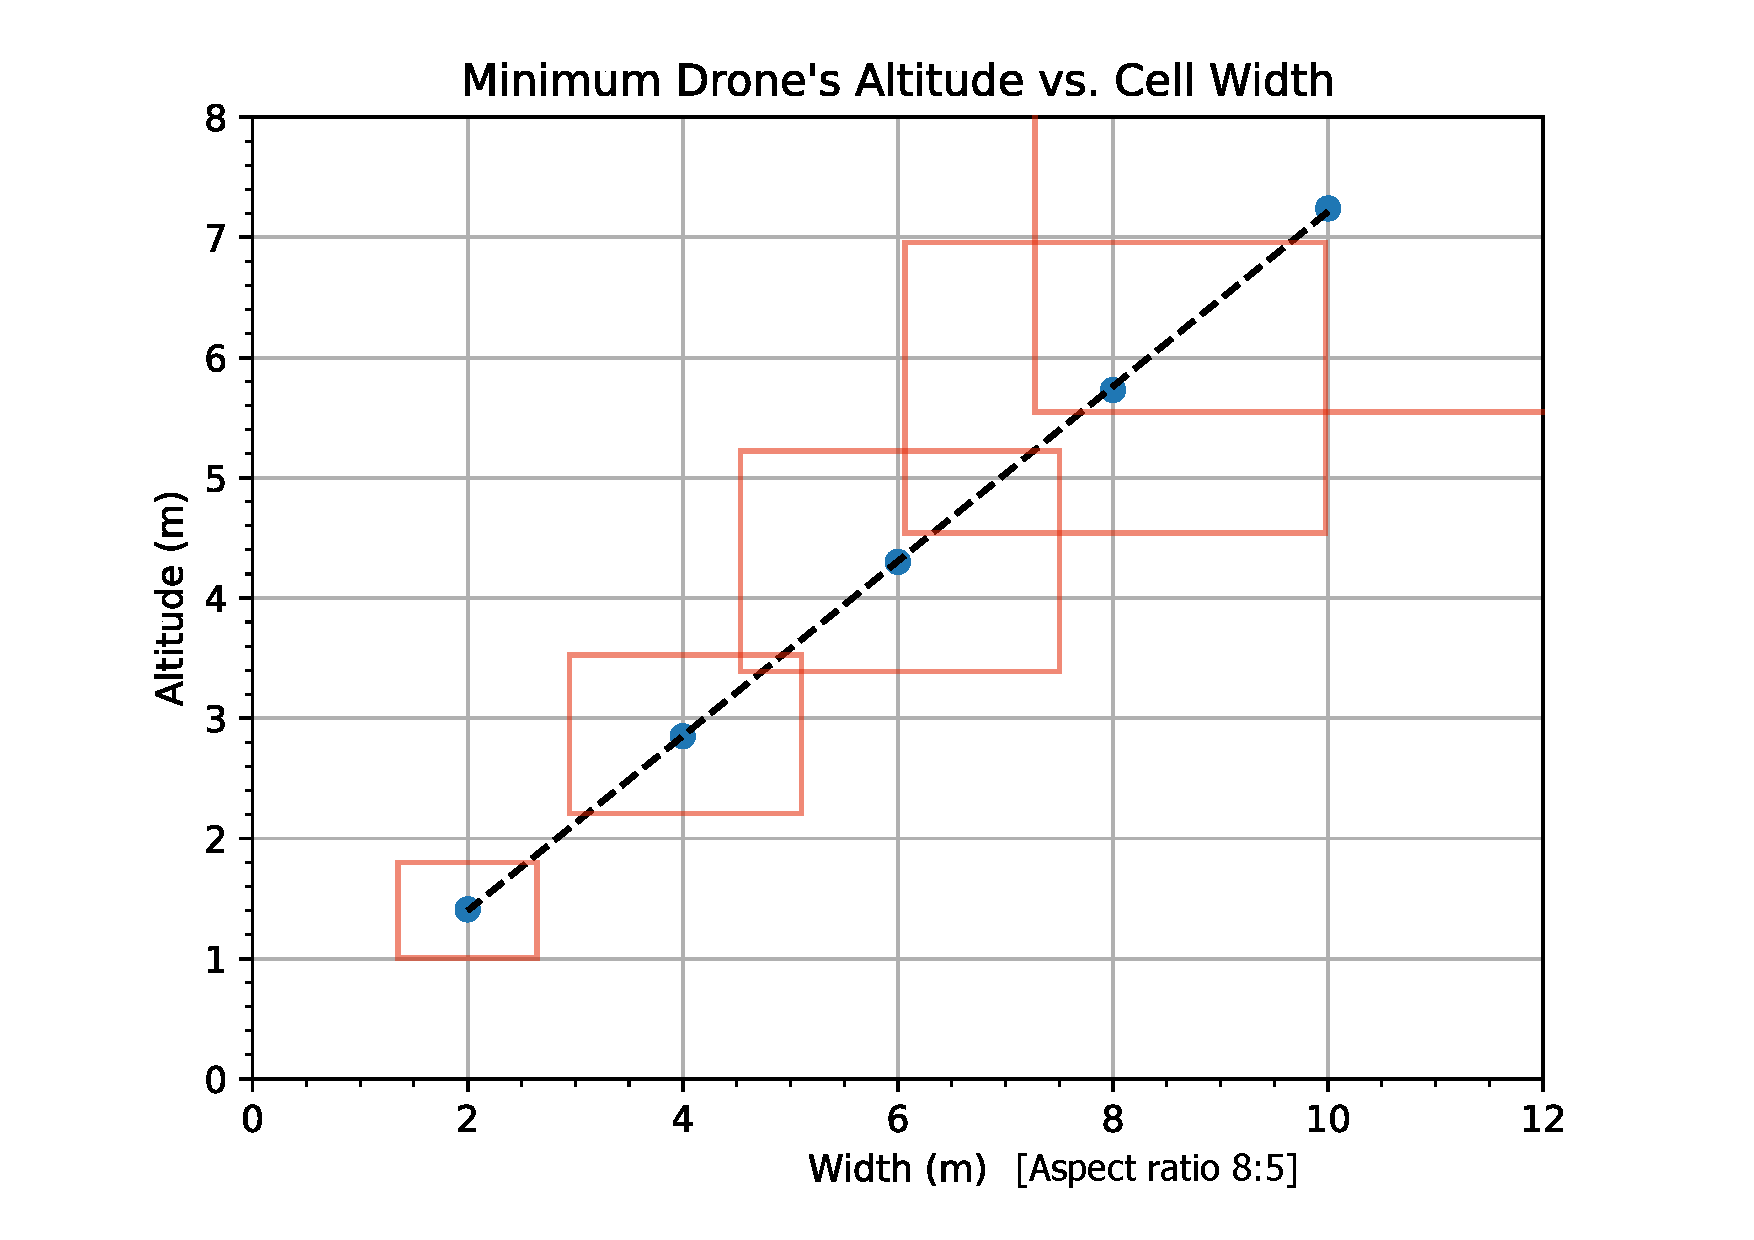
\includegraphics[width=0.8\textwidth]{h-alt}
	\caption{The minimum height that the drone needs to fly at to
        fully cover the cell underneath with the given width.  
        The aspect ratio of each cell is eight-to-five.}
	\label{fig:h-alt}
\end{figure}

To obtain the graph in~\cref{fig:h-alt}, we have flown the drone in
the simulation environment at multiple heights, and below, the ground
was replaced with cells of different sizes as shown
in~\cref{fig:h-alt-ground}.
We then recorded which maximum cell size was the drone able to capture
using its camera and fit a linear regression line through these
points. 

\begin{figure}[tbp]
	\centering
	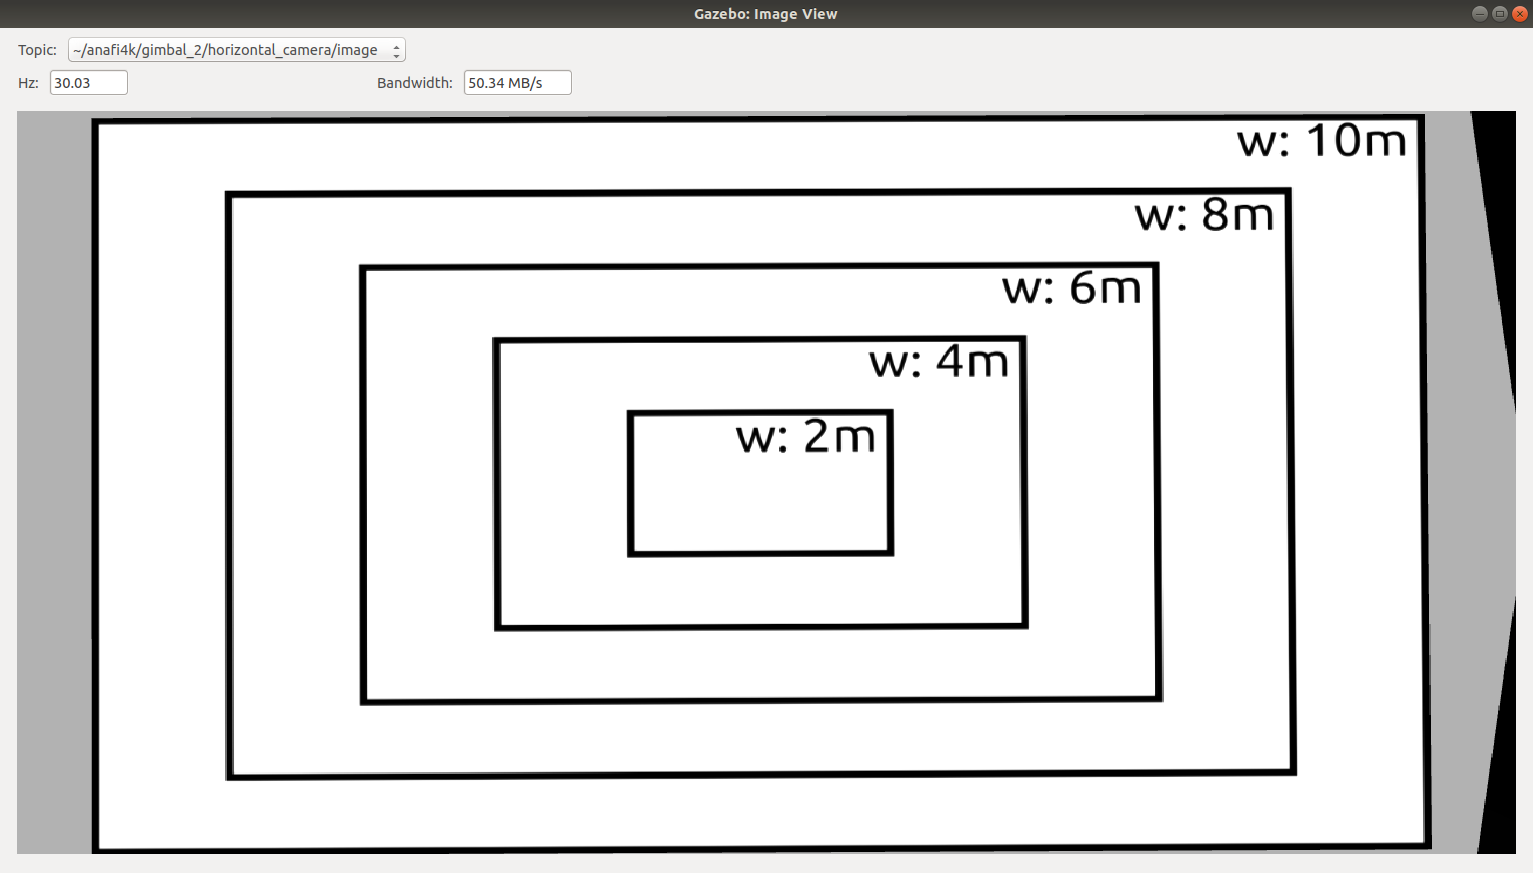
\includegraphics[width=0.8\textwidth]{h-alt-ground}
	\caption{Cells of varying widths as seen by the drone's camera.
        The aspect ratio of all cells is the same which is
        eight-to-five.}
	\label{fig:h-alt-ground}
\end{figure}

\subsection{User interface}

\lipsum[1]

\end{document}
